\documentclass[CMPE]{../KGCOEReport}
\usepackage{float}
\usepackage{adjustbox}
\graphicspath{ {./images/} }

\newcommand{\name}{Mohammed Fareed}
\newcommand{\exerciseNumber}{1}
\newcommand{\exerciseDescription}{Introduction to Vivado \& Simple ALU}
\newcommand{\dateDone}{February 8, 2024}
\newcommand{\dateSubmitted}{February 11, 2024}

\newcommand{\classCode}{CMPE 260}
\newcommand{\LabSectionNum}{4}
\newcommand{\LabInstructor}{Prof.\ Richard Cliver}
\newcommand{\TAs}{Aubrey Tarmu \\ Henry Bang \\ William Tom}
\newcommand{\LectureSectionNum}{2}
\newcommand{\LectureInstructor}{Prof.\ Marcin Lukowiak}


\begin{document}
\maketitle

\section*{Abstract}

In this lab exercise, the functionalities of the Xilinx Vivado Design Suite were explored by designing, implementing, and testing a 4-bit, and later a 32-bit, Arithmetic Logic Unit (ALU) on a Basys3 FPGA. Initially, the project setup included the ALU definition with 'not' and 'shift left logical' operations for a 4-bit design, utilizing a provided testbench for behavioral simulation, and observing synthesis and implementation results. Post-synthesis and post-implementation designs were generated, as well as timing simulations conducted. The project was then scaled to a 32-bit ALU, incorporating additional operations and employing a modified testbench for testing with behavioral timing simulations. The results of the simulations were observed to ensure the ALU's correct operation and timing. The exercise demonstrated the process of designing, implementing, and testing an ALU with the Xilinx Vivado Design Suite.

\section*{Design Methodology}

The design started with a tutorial-guided setup in Vivado, involving project creation, ALU definition, constraint setup, and testbench application. Initially, the ALU supported only 'not' and 'shift left logical' operations for a 4-bit input.

The design was then scaled to a 32-bit ALU, with additional operations including 'and', 'or', 'xor', 'shift right logical', and 'shift right arithmetic'. Figure \ref{fig:alu} shows the block diagram of the designed ALU.

\begin{figure}[H]
    \centering
    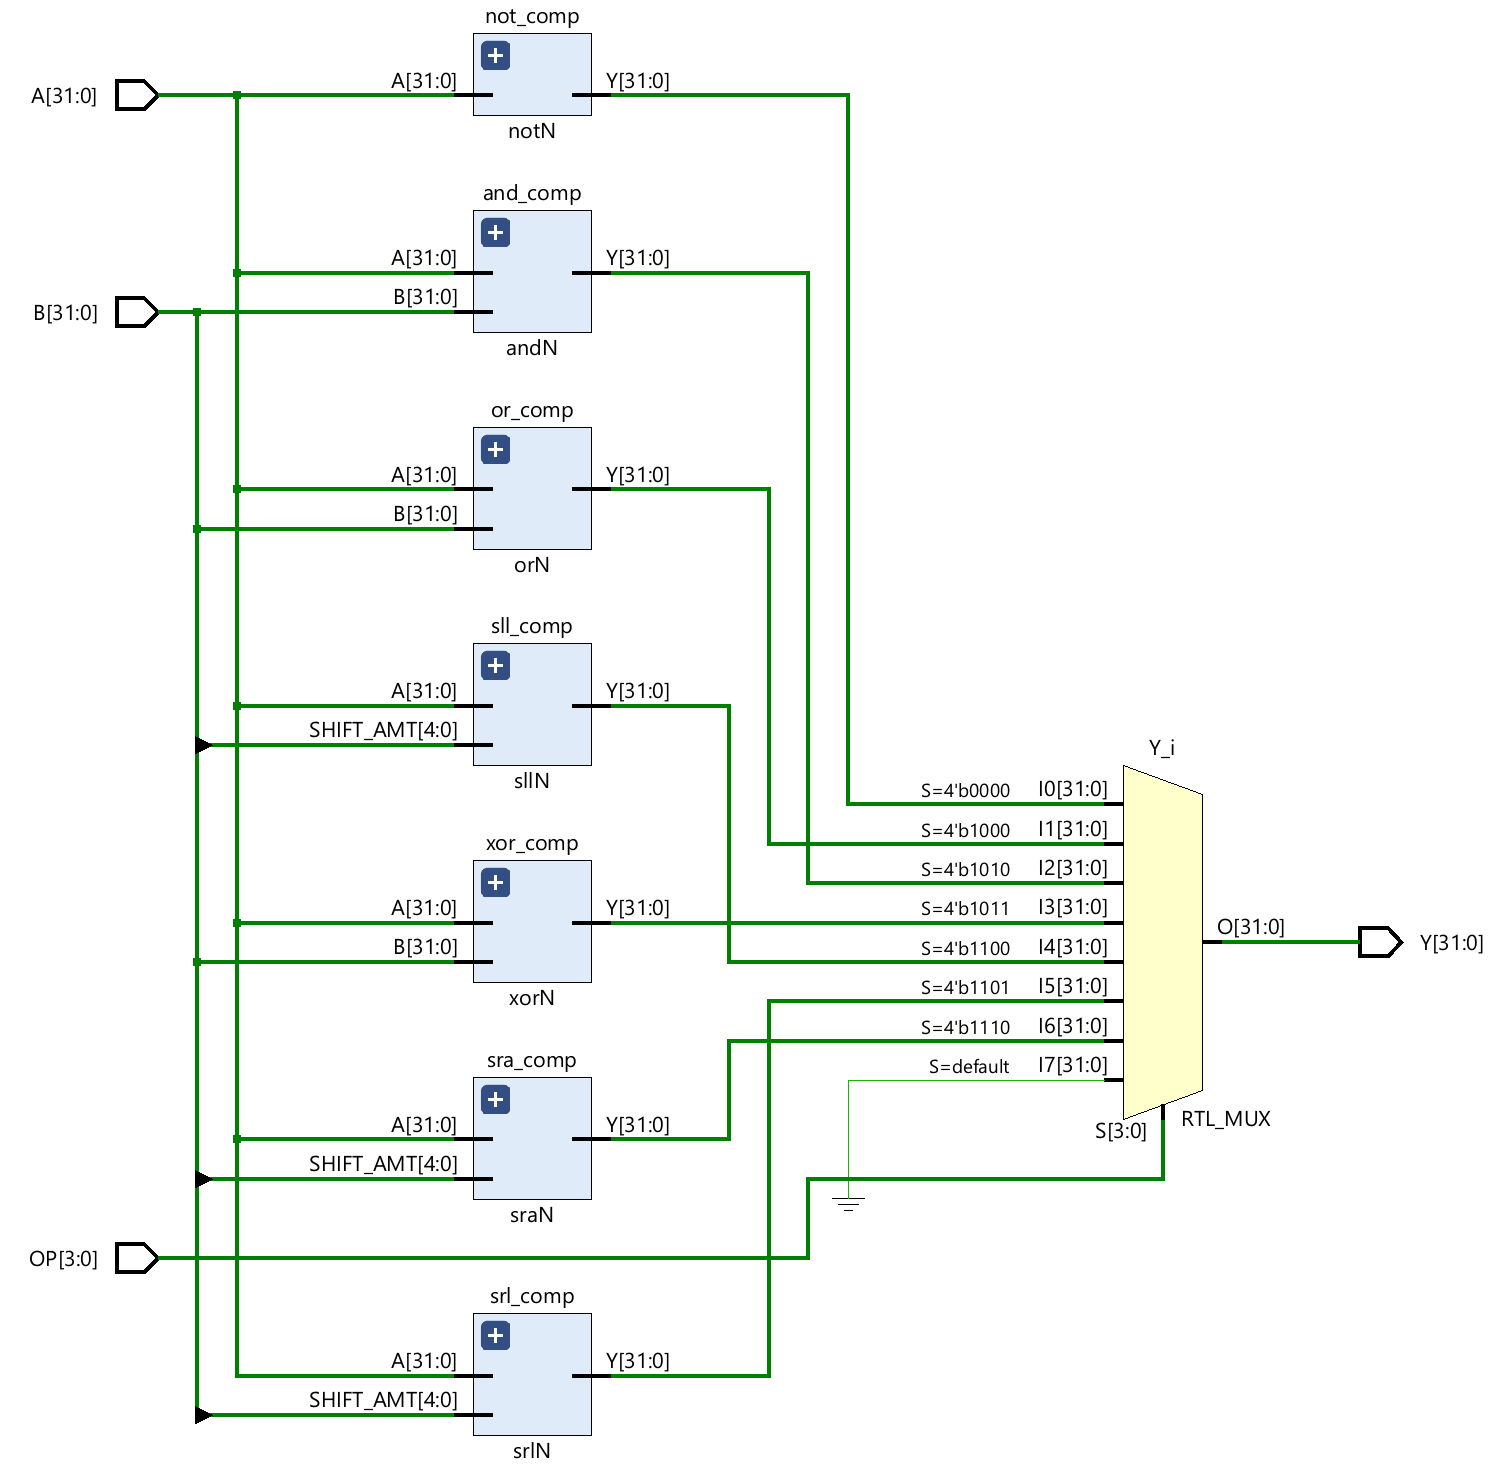
\includegraphics[width=0.6\textwidth]{alu.png}
    \caption{ALU Block Diagram.}
    \label{fig:alu}
\end{figure}

The figure above shows the ALU block diagram, with the inputs and outputs labeled. The diagram shows the ALU's signals and operations, including the 32-bit input, 4-bit operation selection, and 32-bit output. The ALU was implemented using VHDL, with global constants defining the ALU input and shift inputs width. The figure is also applicable to the 4-bit ALU, with the only difference being the input and output widths and the shift input width. Table \ref{tab:operations} shows the operations supported by the ALU.

\begin{table}[H]
    \centering
    \begin{tabular}{|c|c|}
        \hline
        \textbf{OP Code} & \textbf{Operation} \\
        \hline
        0000 & NOT \\
        1010 & AND \\
        1000 & OR \\
        1011 & XOR \\
        1100 & Shift Left Logical \\
        1101 & Shift Right Logical \\
        1110 & Shift Right Arithmetic \\
        \hline
    \end{tabular}
    \caption{ALU Operations.}
    \label{tab:operations}
\end{table}

The operations 'and', 'or', 'xor', and 'not' were implemented using native VHDL operators, while the 'shift left logical' was implemented using a generator that creates a new vector holding vectors of the input vector shifted by all possible amounts, with the shift amount being the index of the vector. The output is then set to the vector indexed with the provided shift amount. The 'shift right logical' and 'shift right arithmetic' operations were implemented using the \verb|shit_right| operator in the \verb|ieee.numeric_std| package. The the logical shift used the unsigned value of the input, while the arithmetic shift used the signed value of the input. The maximum shift amount was defined using a global constant, manually calculated to be equal to \verb|log_2(input_width)|, which is 2 bits for the 4-bit ALU and 5 bits for the 32-bit ALU.\\

The initial 4-bit ALU was redesigned to support 32-bit inputs and outputs by using the global constants to define the input and output widths and generics to define the operation selection width. Generics allowed the design to be scalable, with the 32-bit ALU supporting the same operations as the 4-bit ALU. Changing the global constants from 4 to 32, and vice versa, results in the design scaling to the new width.

\section*{Results and Analysis}

The ALU's functionality was verified through behavioral simulation and post-implementation timing simulation. The initial 4-bit design and the enhanced 32-bit design were both tested. The testbench for testing was modified such that a vector of test cases was used to test the ALU's operations, with the expected results being compared to the actual results. Assertions were used to verify the results, reporting an error if the expected and actual results did not match.

4-bit test cases were first used to test the 4-bit ALU. Figure \ref{fig:4bit_behavior} shows the behavioral simulation results for the 4-bit ALU.

\begin{figure}[H]
    \centering
    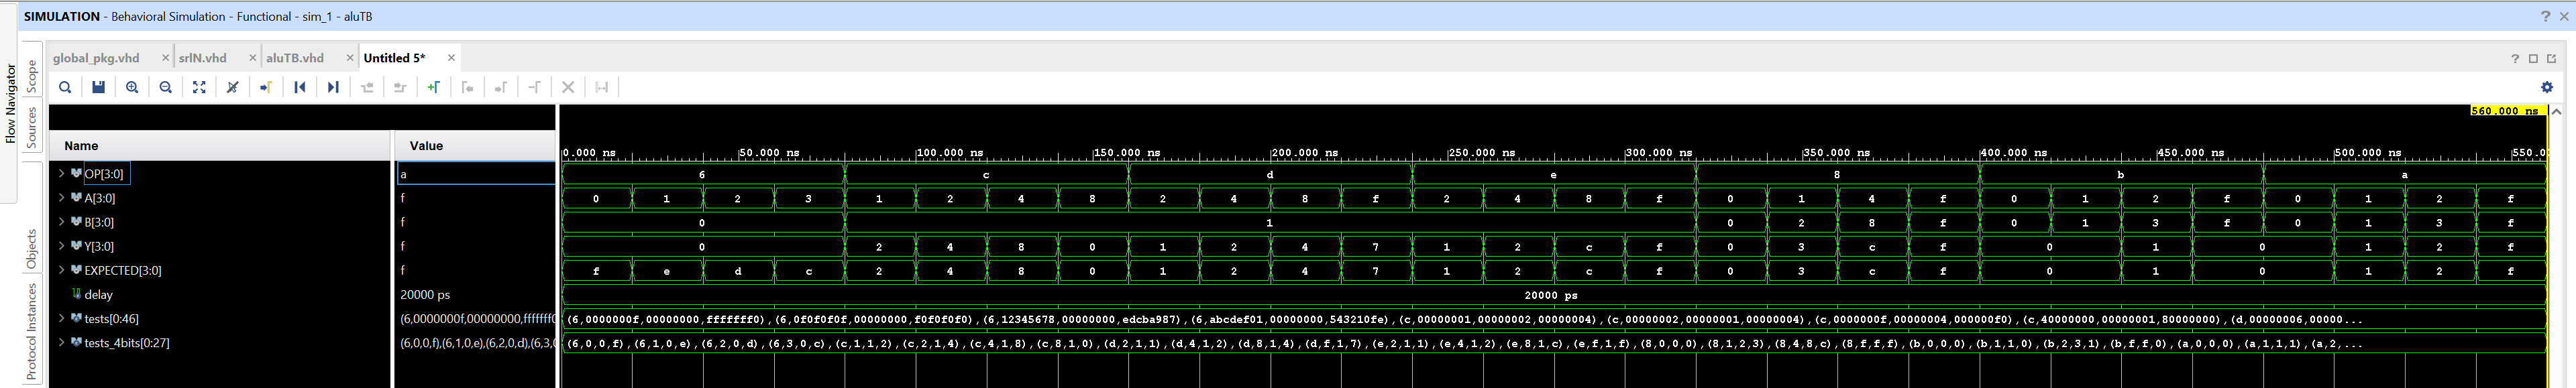
\includegraphics[width=1\textwidth]{behavior.png}
    \caption{4-bit ALU Behavioral Simulation Results.}
    \label{fig:4bit_behavior}
\end{figure}

The waveform displayed in the figure shows the result \verb|Y| matching the expected output for each operation. The testbench was run, and the results were verified to match the expected results. For example, at time 260 ns, the operation \verb|sra| was performed, with the input \verb|A| being \verb|4 = 0100| and the shift amount being \verb|1|. The expected result was \verb|2 = 0010|, and the actual result was \verb|0010|, as shown in the waveform.

Post-synthesis and post-implementation designs were generated for the 4-bit ALU, with the results of the timing simulations shown in Figures \ref{fig:4bit_synthesis} and \ref{fig:4bit_implementation}.

\begin{figure}[H]
    \centering
    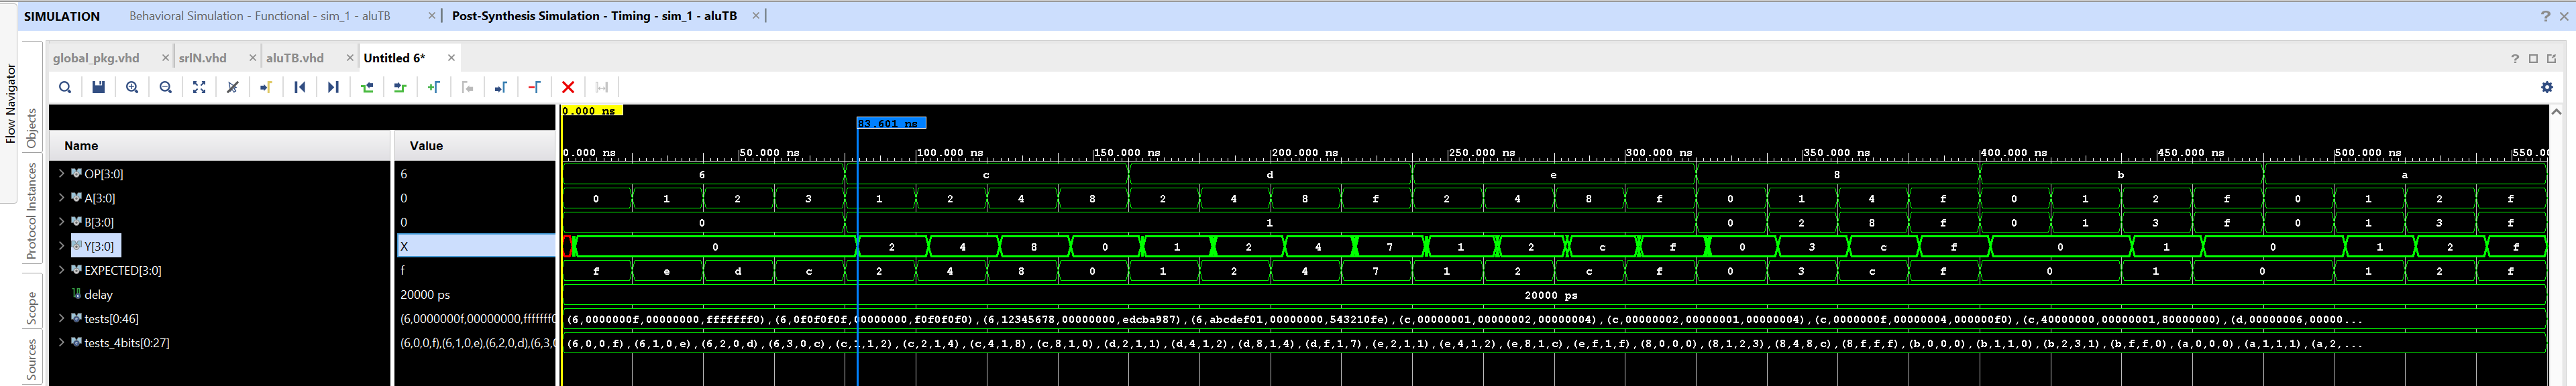
\includegraphics[width=1\textwidth]{synth.png}
    \caption{4-bit ALU Synthesis Timing Results.}
    \label{fig:4bit_synthesis}
\end{figure}

\begin{figure}[H]
    \centering
    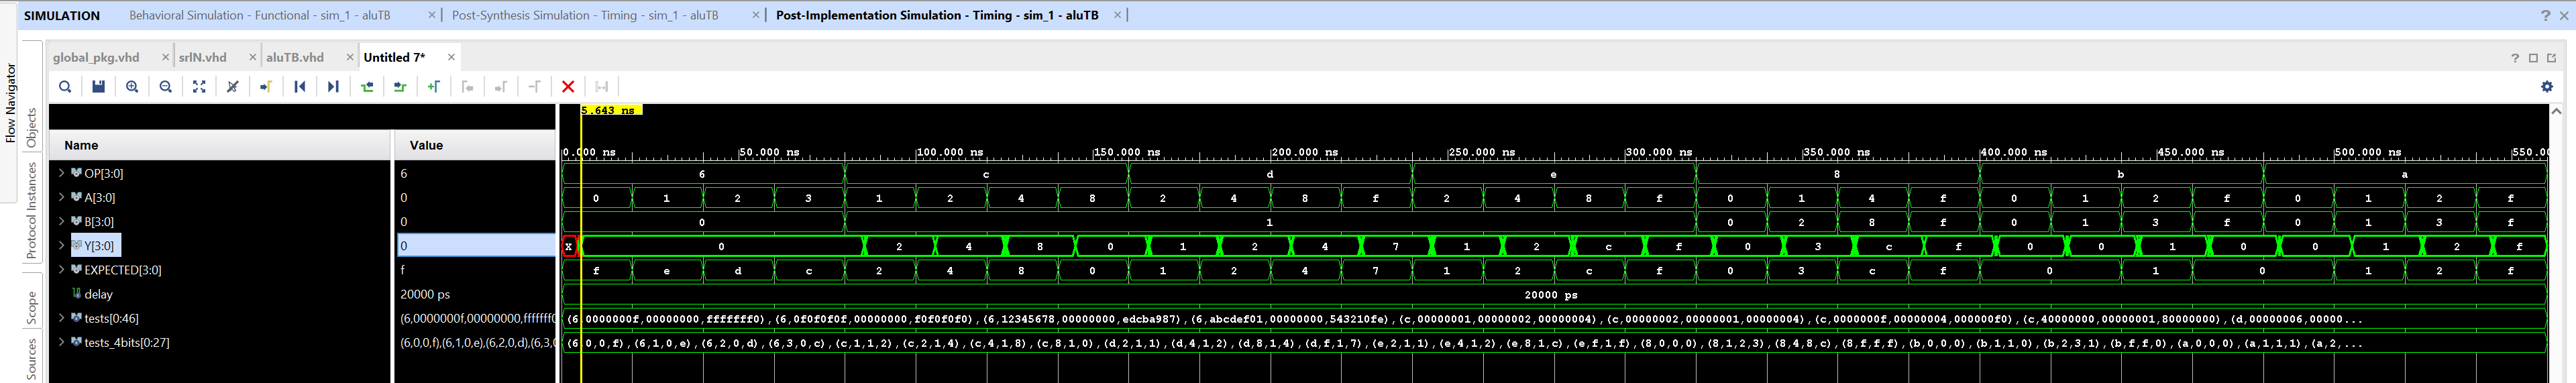
\includegraphics[width=1\textwidth]{implement.png}
    \caption{4-bit ALU Implementation Timing Results.}
    \label{fig:4bit_implementation}
\end{figure}

The timing results in the figures show the ALU's operations matching the behavioral simulation, with a delay in the output being around 3.6 ns. The results indicate that the ALU's operations are functional and reliable given the operation time and delay.

The 32-bit ALU was then tested using the modified testbench, with the results of the behavioral simulation shown in Figure \ref{fig:32bit_behavior}.

\begin{figure}[H]
    \centering
    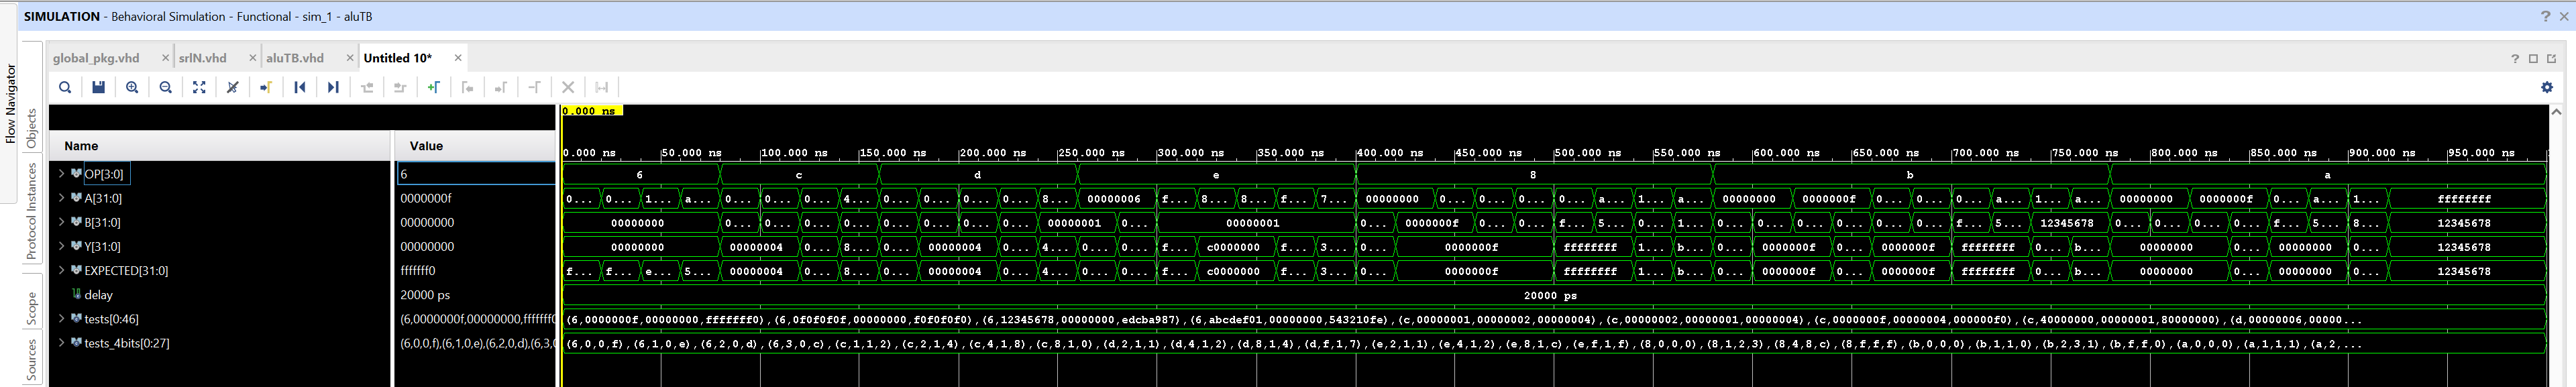
\includegraphics[width=1\textwidth]{behavior2.png}
    \caption{32-bit ALU Behavioral Simulation Results.}
    \label{fig:32bit_behavior}
\end{figure}

The waveform displayed in the figure shows the result \verb|Y| matching the expected output for each operation. For example, at time 420 ns, the operation \verb|OR| was performed, with the input \verb|A| being \verb|0x0| and the input \verb|B| being \verb|0xf|. The expected result was \verb|0xf|, matching the actual result \verb|0xf|, as shown in the waveform.

The post-synthesis and post-implementation designs were generated for the 32-bit ALU, with the results of the timing simulations shown in Figures \ref{fig:32bit_synthesis} and \ref{fig:32bit_implementation}.

\begin{figure}[H]
    \centering
    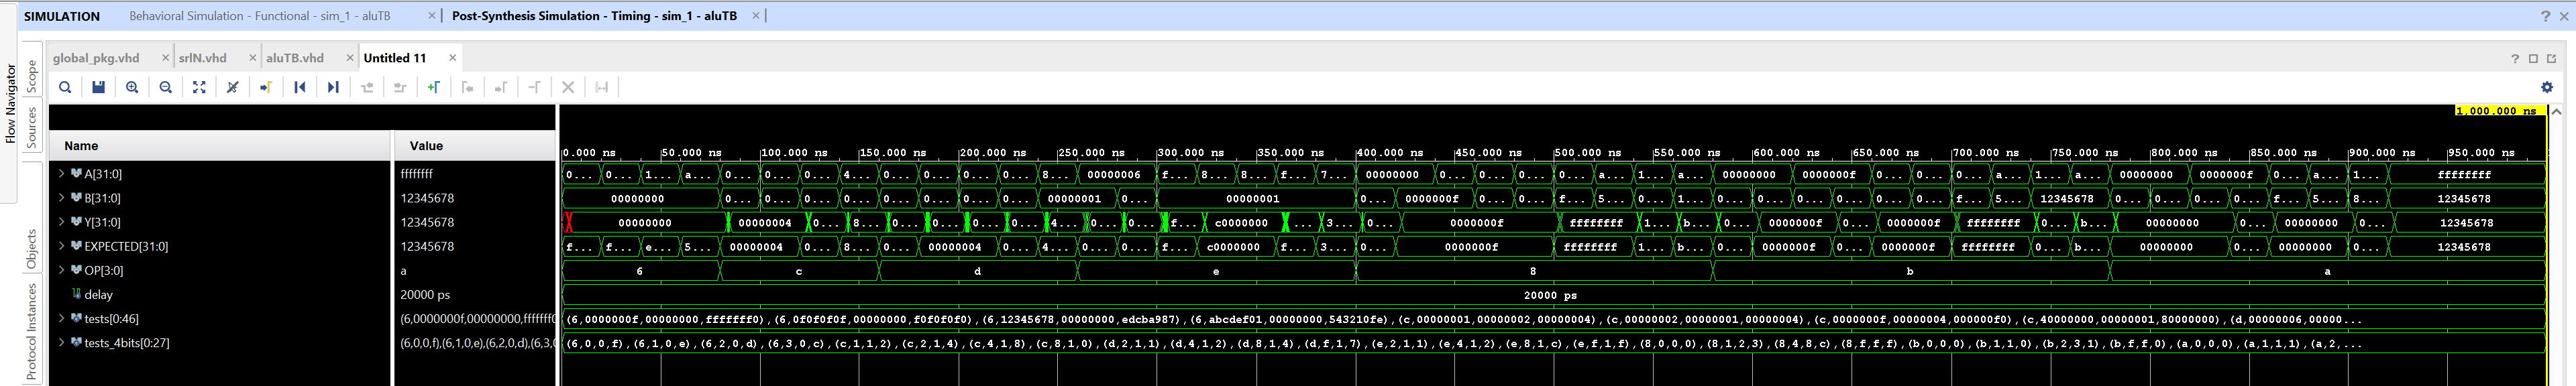
\includegraphics[width=1\textwidth]{synth2.png}
    \caption{32-bit ALU Synthesis Timing Results.}
    \label{fig:32bit_synthesis}
\end{figure}

\begin{figure}[H]
    \centering
    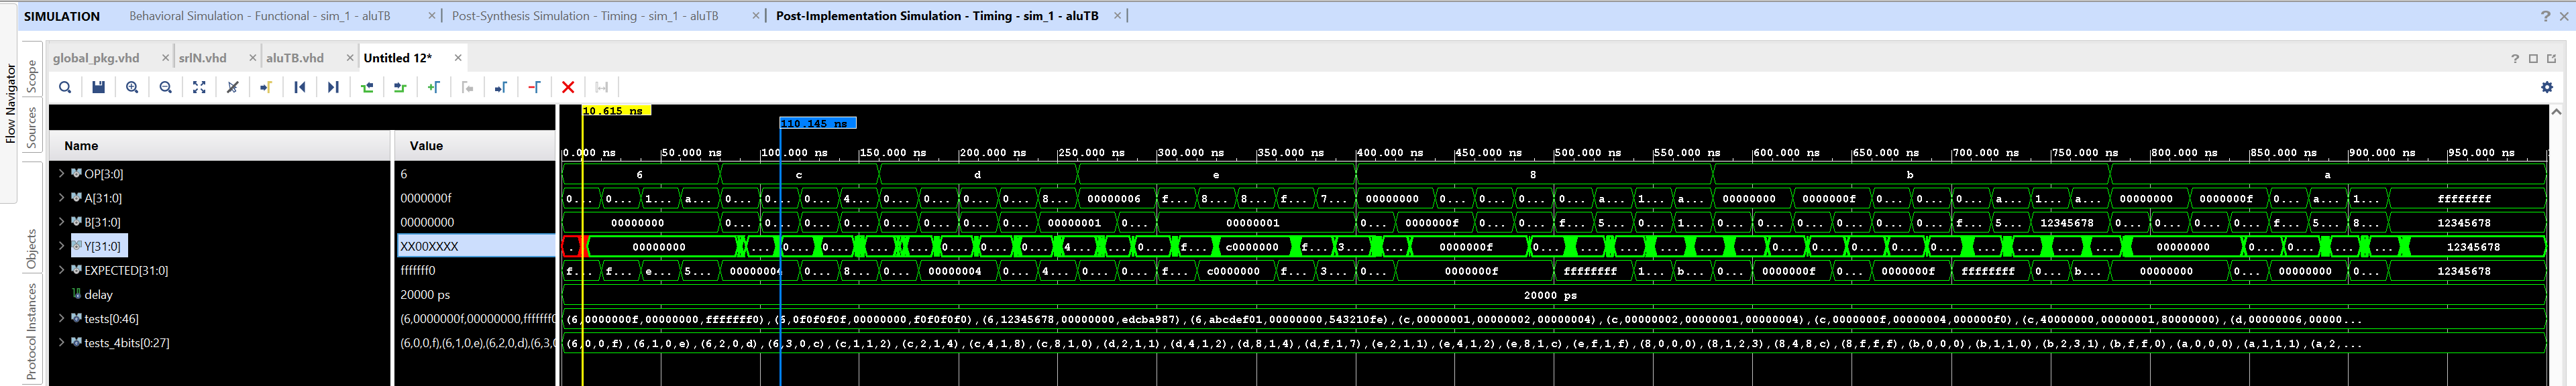
\includegraphics[width=1\textwidth]{implement2.png}
    \caption{32-bit ALU Implementation Timing Results.}
    \label{fig:32bit_implementation}
\end{figure}

The timing results in the figures show the ALU's operations matching the behavioral simulation, with a delay in the output being around 10.145 ns. The results indicate that the ALU's operations are functional and reliable given the operation time and delay.\\

The testbench was designed such that a record is created that holds the operation, inputs, and expected output. Two vectors were then created that hold the different test cases, one vector with 32-bit inputs and the other with 4-bit inputs. The testbench then iterates through the vectors, performing the operations and comparing the expected and actual results. The testbench was designed to be scalable, with the 32-bit ALU using the same testbench as the 4-bit ALU. Four test cases were used for each operation, with the 32-bit ALU including additional edge cases.

\section*{Conclusion}

This exercise successfully demonstrated the process of designing, implementing, and testing an ALU with the Xilinx Vivado Design Suite. Starting from a basic 4-bit ALU, the project was scaled to a more complex 32-bit version, with the design verified through extensive testing. The results of the behavioral, synthesis, and implementation simulations indicated that the ALU's operations were functional and reliable, with the 32-bit ALU supporting the same operations as the 4-bit ALU. The exercise provided a comprehensive understanding of the Vivado Design Suite and the process of designing and testing an ALU.

\newpage
\begin{figure}[H]
    \centering
    \begin{adjustbox}{center}
        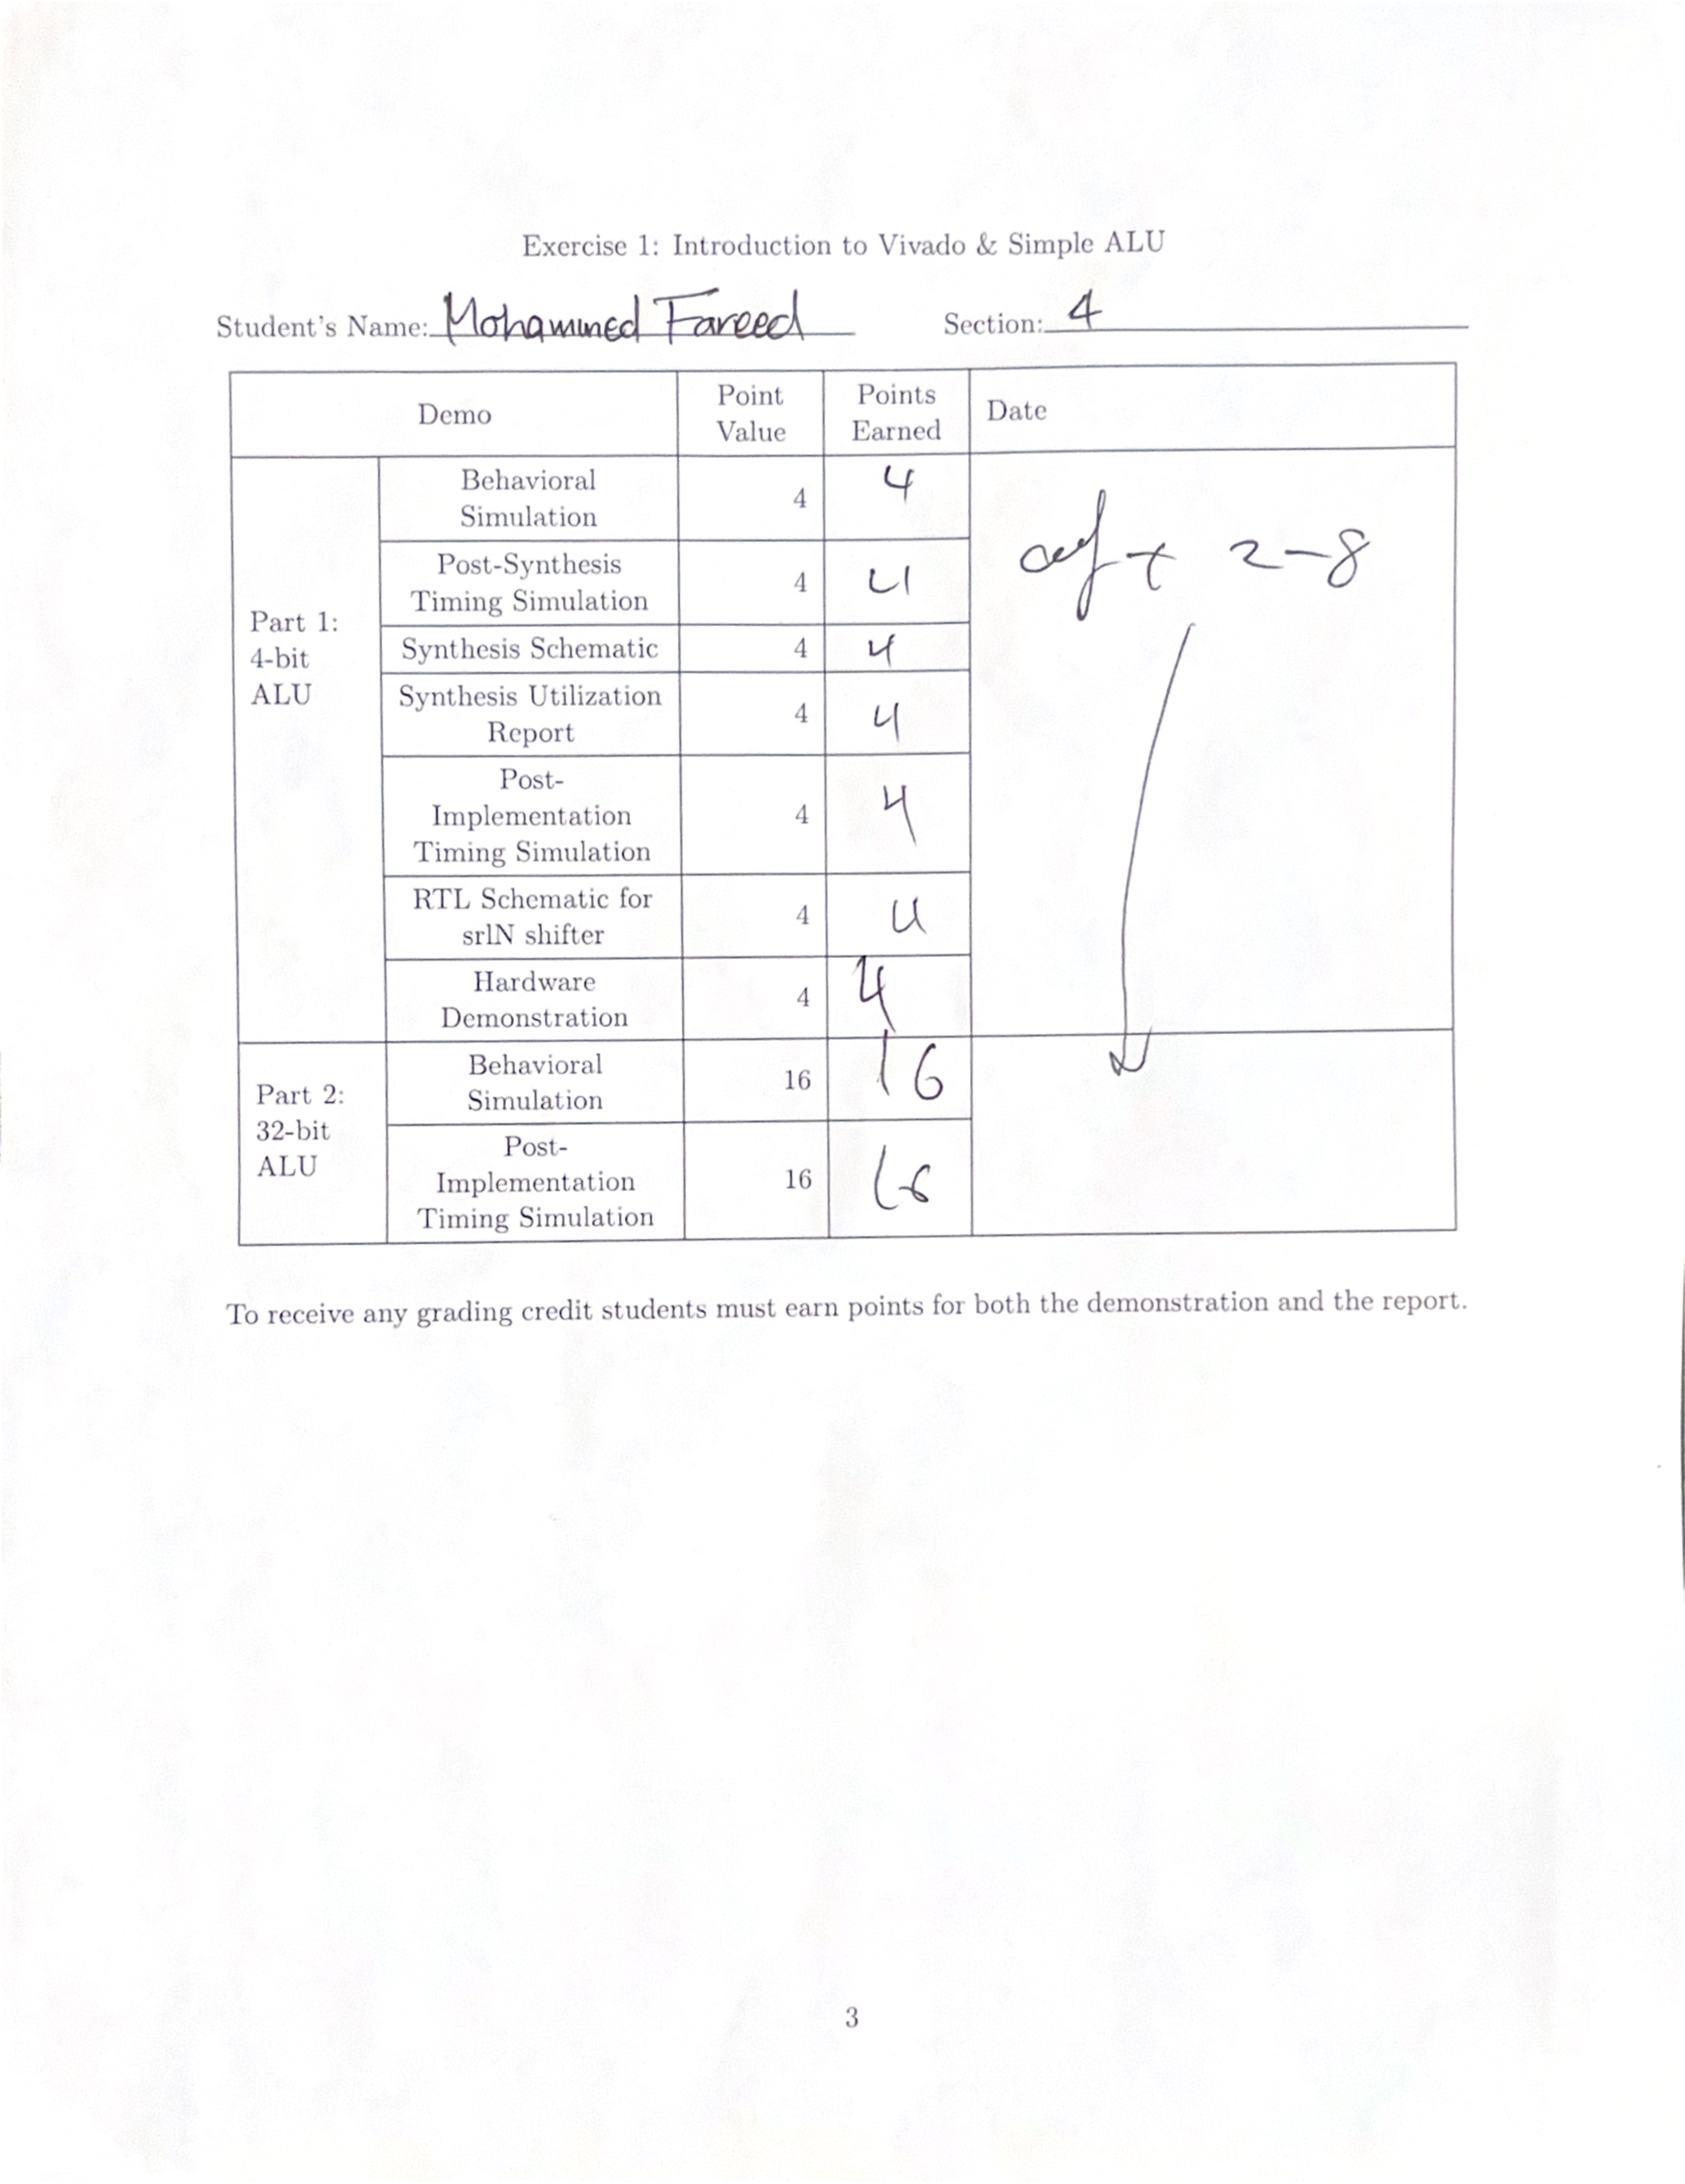
\includegraphics[width=1.35\textwidth]{signoff.pdf}
    \end{adjustbox}
\end{figure}

\end{document}
